
%(BEGIN_QUESTION)
% Copyright 2012, Tony R. Kuphaldt, released under the Creative Commons Attribution License (v 1.0)
% This means you may do almost anything with this work of mine, so long as you give me proper credit

This elevator control system has a problem.  No matter which pushbutton is pressed, the elevator remains ``stuck'' in the full-down position.  The following pictorial diagram shows the wiring of this system, along with the I/O card status lights as they appear with no one pressing any pushbuttons:

$$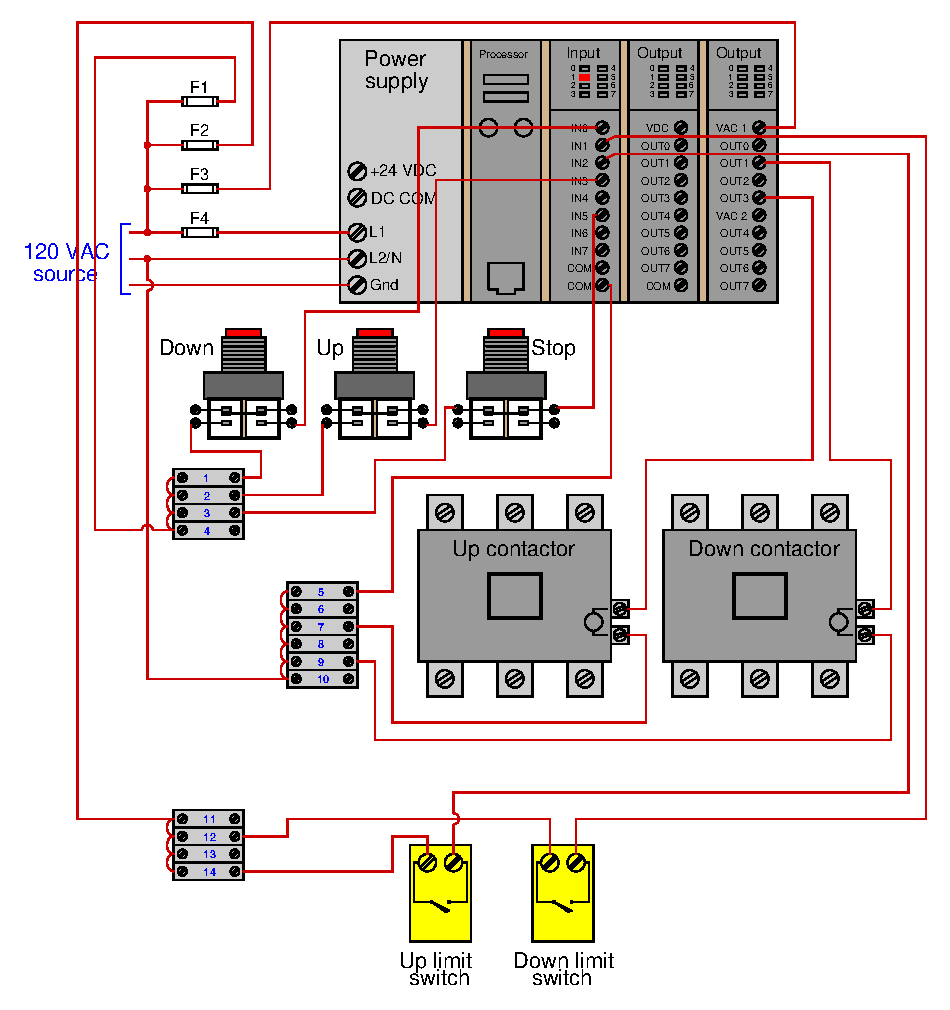
\includegraphics[width=15.5cm]{i02539x01.eps}$$

\vskip 10pt

Based on this information, determine a likely fault causing this elevator to remain stuck at the full-down position.

\underbar{file i02539}
%(END_QUESTION)





%(BEGIN_ANSWER)

The PLC is not seeing the signal it needs to from the NC ``Stop'' pushbutton, and so it ``thinks'' someone is pressing the Stop pushbutton.  Possible faults include:

\begin{itemize}
\item{} Stop pushbutton switch failed open
\item{} Open wire fault from Stop pushbutton to IN5 terminal
\item{} Open wire fault from terminal 3 to Stop pushbutton
\item{} Open wire fault from terminal 4 to fuse F1
\item{} Fuse F1 blown
\end{itemize}

%(END_ANSWER)





%(BEGIN_NOTES)


%INDEX% PLC, troubleshooting: elevator control system

%(END_NOTES)


